\documentclass[12pt, a4paper]{extarticle}

\usepackage[english, russian]{babel}
\usepackage[utf8]{inputenc}
\usepackage{amsmath}
\usepackage{amssymb}
\usepackage{graphicx}
\usepackage{multicol}
\usepackage[12pt]{extsizes}
\usepackage{listingsutf8}
\usepackage{color}
\usepackage{wrapfig}
\usepackage{enumerate}
\usepackage{amsthm}
\usepackage{indentfirst}
\usepackage{tabularx,lipsum,environ,amsmath,amssymb}
\usepackage{multirow}

\usepackage{setspace}
\singlespacing
\onehalfspacing
\doublespacing

\allowdisplaybreaks
\binoppenalty = 10000
\relpenalty = 10000
\textheight = 23cm
\textwidth = 20cm
\oddsidemargin = 0pt
%\topmargin = -1.5cm
\parskip = 0pt
\tolerance = 2000
\flushbottom

\usepackage[left=30mm, right=20mm, top=20mm, bottom=30mm, nohead, footskip=10mm]{geometry}
% bottom=2cm, bindingoffset=0cm]

\makeatletter
\newcommand{\problemtitle}[1]{\gdef\@problemtitle{#1}}% Store problem title
\newcommand{\probleminput}[1]{\gdef\@probleminput{#1}}% Store problem input
\newcommand{\problemquestion}[1]{\gdef\@problemquestion{#1}}% Store problem question
\NewEnviron{problem}{
  \problemtitle{}\probleminput{}\problemquestion{}% Default input is empty
  \BODY% Parse input
  \par\addvspace{.5\baselineskip}
  \noindent
  \begin{tabularx}{\textwidth}{@{\hspace{\parindent}} l X c}
    \multicolumn{2}{@{\hspace{\parindent}}l}{\@problemtitle} \\% Title
    \textbf{Дано:} & \@probleminput \\% Input
    \textbf{Найти:} & \@problemquestion% Question
  \end{tabularx}
  \par\addvspace{.5\baselineskip}
}

\pagestyle{plain}

\renewcommand{\thesection}{\arabic{section}}

\begin{document}

\allowdisplaybreaks[1]

\begin{titlepage}
\setstretch{1}
\begin{center}
\ \vspace{-1.5cm}

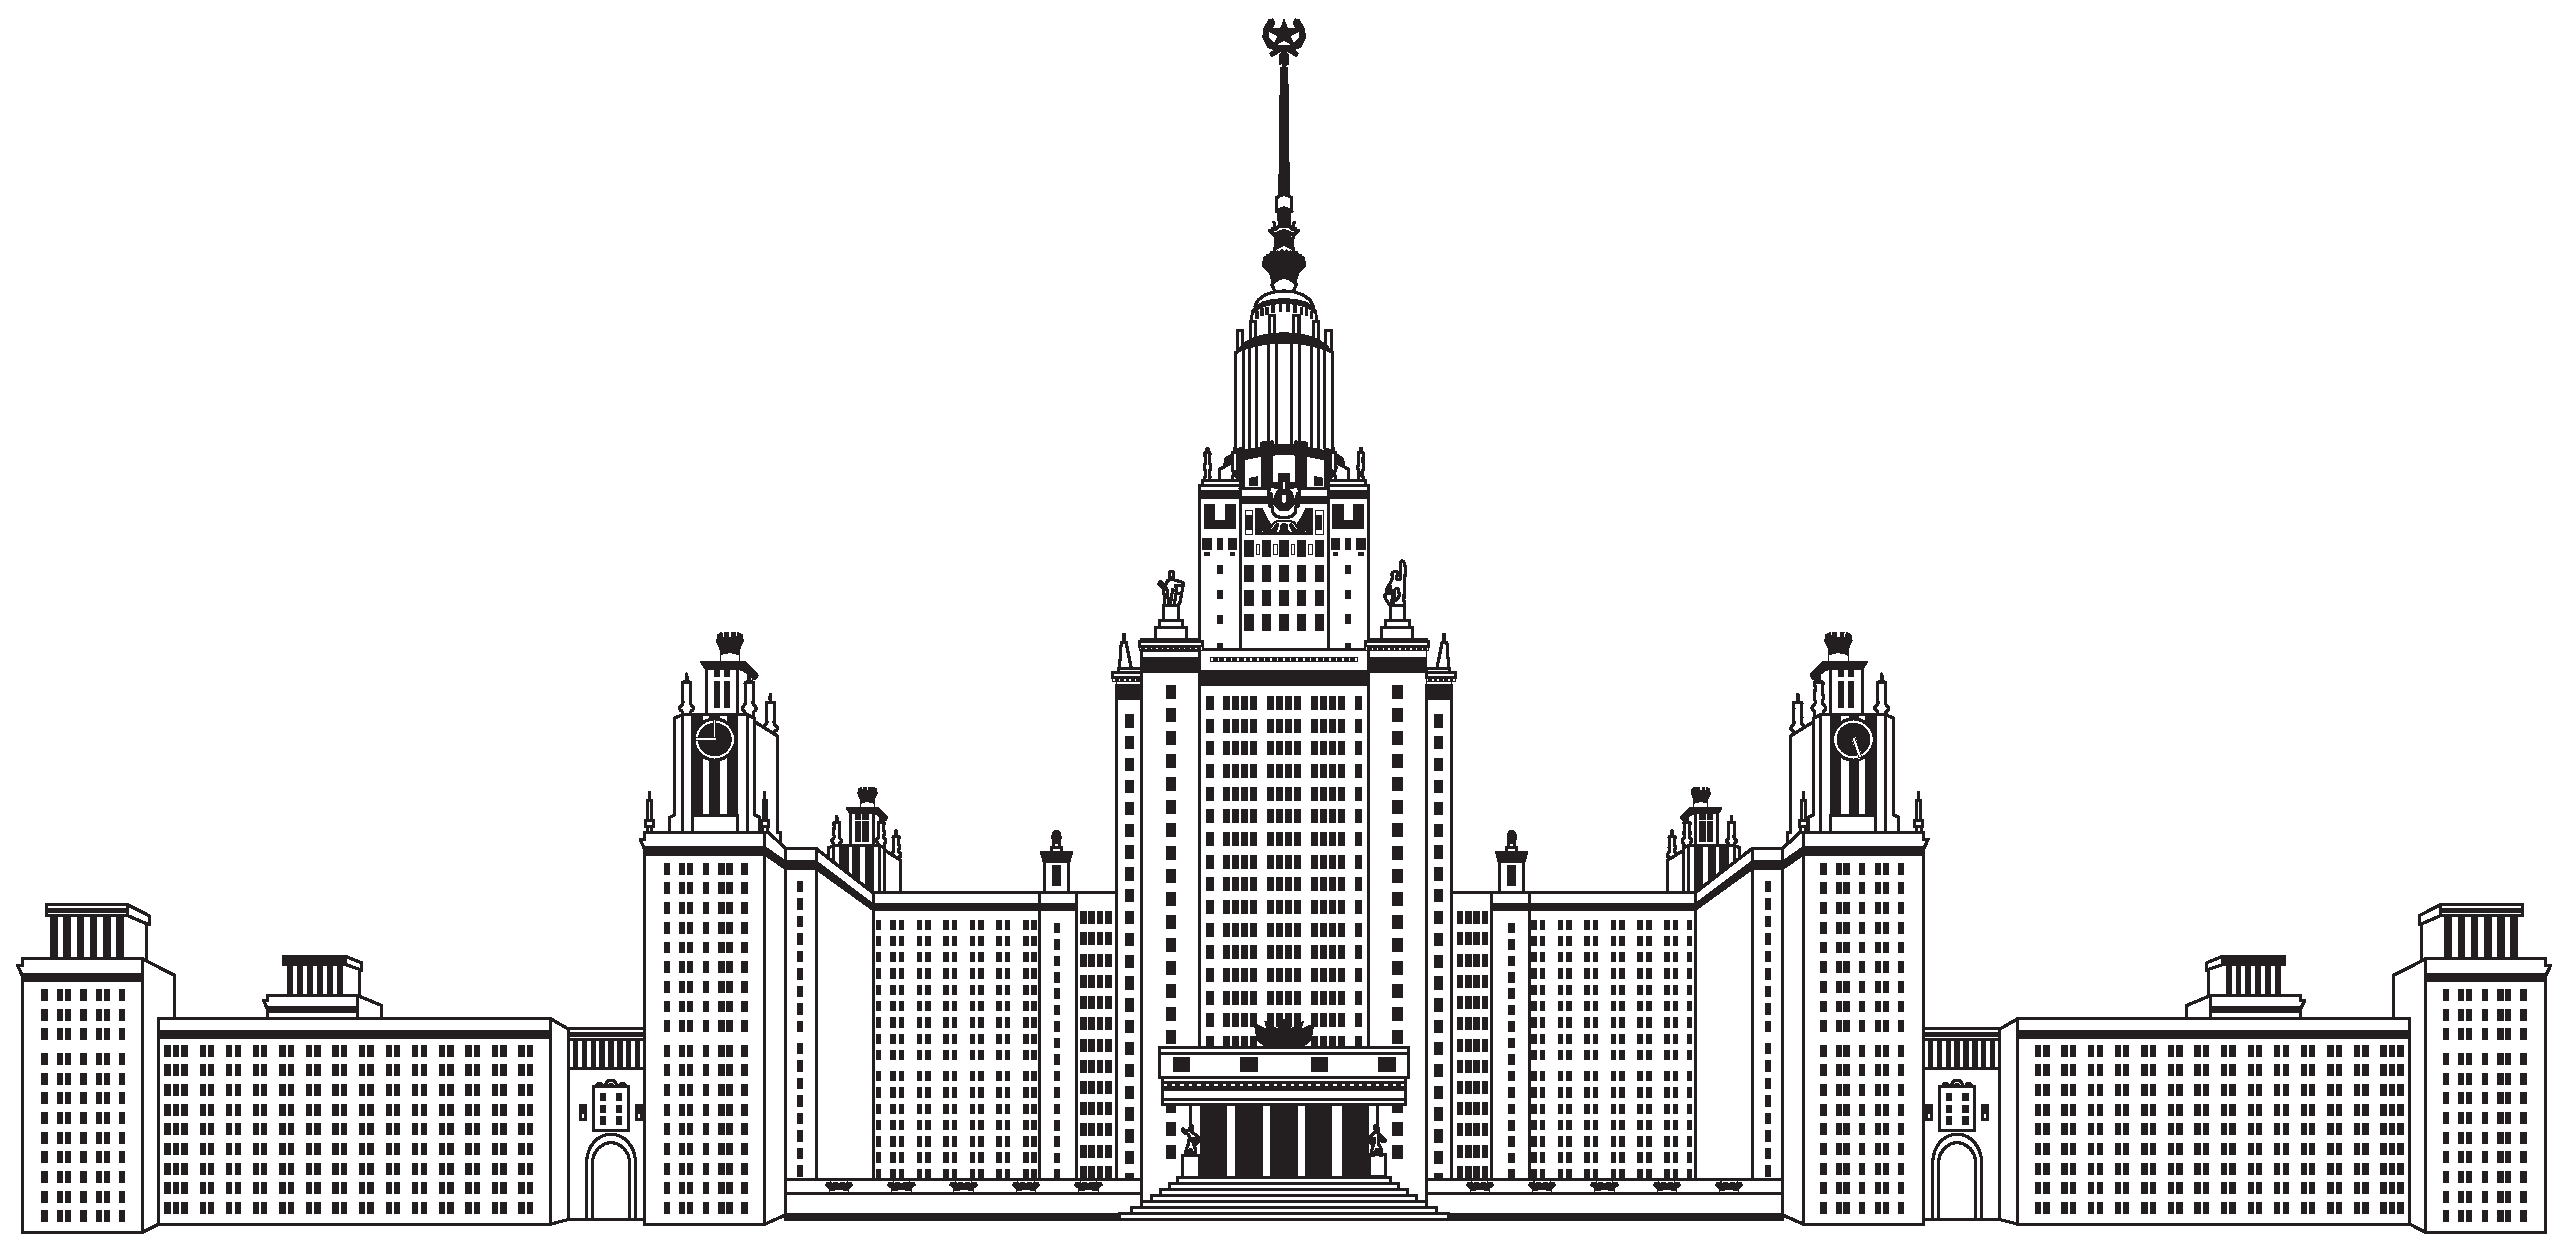
\includegraphics[width=0.5\textwidth]{data/images/msu_logo.eps}\\
{ Московский государственный университет имени М.В. Ломоносова \\
Факультет вычислительной математики и кибернетики\\
Кафедра исследования операций}

\vspace{3cm}

{\Large Лаврухин Ефим Валерьевич}

\vspace{1cm}

{\Large\bfseries
Применение нейронных сетей для решения задачи оптимальной сегментации томографических
изображений геологических пород\\}

\vspace{1cm}

{\textbf \large МАГИСТЕРСКАЯ ДИССЕРТАЦИЯ}
\end{center}

\vfill

\begin{flushright}
  \textbf{Научный руководитель:}\\
  к.ф.-м.н., доцент\\
  Д.В.~Денисов
\end{flushright}

\vfill

\begin{center}
Москва, 2018
\end{center}

\vspace{1cm}

\enlargethispage{2\baselineskip}

\end{titlepage}

\setstretch{1.5}

\newpage

\tableofcontents

\newpage


\section{Введение} \label{intro}

В настоящее время добыча полезных ископаемых требует большое количество 
данных о разрабатываемых породах-коллекторах. Эти данные получают в том числе с помощью методов цифровой петрофизики, которые работают с  
2-D или 3-D изображениями, сделанными с помощью рентгеновской томографии \cite{1}. Большинство изображений строения пород представлены в градациях серого, которые указывают на интенсивность поглощения рентгеновских лучей. На практике любой метод численного расчета характеристик исходных пород состоит из нескольких отдельных этапов. 
И первый этап -- это сегментация входного изображения, разделение его
на несколько различных фаз по плотности вещества. В простейшем случае выполняется бинаризация -- разделение на твёрдую породу и поры \cite{2}. 

Существует большое количество методов сегментации. Они существенно отличаются в принимаемых предположениях о входных изображениях и используемом математическом аппарате: градиентные \cite{13}, морфологические \cite{17}, случайные поля \cite{14}, методы Монте-Карло \cite{16}. У этих методов есть ряд достоинств: присутствует математическая формализация, относительная простота постановки задачи, интерпретируемость результатов. Но в то же время все они обладают серьёзным недостатком -- в них присутствуют гиперпараметры, которые сильно влияют на качество результата. Это делает затруднительным их применение без оператора, который контролирует процесс и подбирает нужные значения параметров для  конкретных входных данных. 

Относительно недавно появились методы сегментации с использованием машинного обучения. Классические методы машинного обучения уже применялись в сегментации изображений геологических пород \cite{3}, \cite{4}, \cite{5}.

Сейчас свёрточные нейронные сети являются, фактически, state-of-the-art в задачах обрабоки изображений и используются во многих прикладных областях: биологии \cite{6}, медицине \cite{18}, распознавании образов \cite{11}. На текущий момент выпущено достаточно много работ, в которых исследуются методы глубинного обучения для решения связанных с сегментацией пород задач. В частности для  построения стохастической реконструции пород с последующим моделированием физических свойств \cite{7}, \cite{8}, \cite{9}, \cite{10}. Но статей, в которых глубинное обучение применяется для сегментации геологических пород, крайне мало. 

Цель данной работы -- построить модель для сегментации томографических изображений гелогогических пород, которая бы имела высокое качество работы и не была бы чувствительной к настройке оператором. В данной работе модель будет строится с помощью методов глубинного обучения, которые, как говорилось ранее, зарекомендовали себя в похожих задача. В качестве модели будет использоваться полносвёрточная нейронная сеть.

В ходе работы решались следующие задачи:
\begin{enumerate}
	\item Постановка задачи оптимальной сегментации как задачи нелинейной оптимизации(гл. \ref{seg_all}).
	
	\item Выбор полносвёртночной архитектуры нейронной сети для  выполнения сегментацию изображений томограмм(гл. \ref{seg_nn}).

	\item Построение стабильного алгоритма обучения сети(гл. \ref{seg_optimization}).
	
	\item Решение проблемы отсутствия размеченных обучающих данных(гл. \ref{seg_tasks}).
	
	\item Проверка модели на реальных данных(гл. \ref{seg_results}).
	
	\item Анализ полученных результатов(гл. \ref{conclusion}). 
	
\end{enumerate}
  
\newpage


\section{Cегментации изображений геологических пород} \label{seg_all}

В данной главе будет формально поставлена практическая задача сегментации 
томографических изображений геологических пород: самая общая постановка(п. \ref{seg_def}) и постановки, которые используются  в данной работе (п. \ref{seg_features}, \ref{seg_supervised}).
 
\subsection{Постановка задачи сегментации} \label{seg_def}

Рассмотрим простейшую постановку задачи сегментации изображения.

\begin{problem}
  \problemtitle{\textbf{Задача сегментации изображения}}
  \probleminput{изображение 
	$S = (s_{ij})_{i=1, j=1}^{H, W},\ s_{ij} \in [0, 1]$, где 
$H$ -- высота изображения, $W$ -- ширина изображения.}
  \problemquestion{для каждого пикселя соответствующий ему сегмент изображения, 
т.е. соответствие $s_{ij} \rightarrow m_{ij},\ m_{ij} \in C = \{ 0, ... , N_c-1 \} $,
где $N_c$ -- число различных сегментов.
}
\end{problem}

Подразумевается, что для каждого изображения $S$ существует 
истинное(возможно, не одно) сегментированное изображение $M = (m_{ij})_{i=1, j=1}^{H, W}$.
Поэтому можно перейти к следующей постановке задачи: найти алгоритм сегментации $\mathcal{A}$, такой, что он преобразует любое 
изображение $S$ в  маску $\hat{M}$:
\begin{equation} \label{unsupervised}
	\mathcal{A}(S | \theta) = \hat{M}
\end{equation} 
, где $\theta$ -- настраеваемые параметры нашего алгоритма.

Для задачи возникают следующие вопросы:
\begin{enumerate}
	\item Как выбрать алгоритм $\mathcal{A}$?
	\item Как настроить параметры $\theta$?
	\item Как оценить ошибку алгоритма?
\end{enumerate}
Существуют различные способы рещения этих вопросов.
Выбор алгоритма $\mathcal{A}$ и способа оценки качества его работы обуславливается задачей и необходимыми результатами. 
Подбор параметров $\theta$ выполняется непосредственно 
оператором, с помощью 
обучения без учителя(unsupervised learning) или с помощью обучения с учителем(supervised learning).

\newpage

\subsection{Задача сегментации геологических пород} \label{seg_features}

Для задачи сегментации томографических изображений геологических пород существуют некоторые особенности. 

\begin{problem}
  \problemtitle{\textbf{Задача сегментации томографических изображений}}
  \probleminput{исходный стек изображений 
	$S = (s_{ijk})_{i=1, j=1, k=1}^{H, W, D},\ s_{ijk} \in [0, 1]$, где 
$H$ -- высота изображения, $W$ -- ширина изображения, $D$ -- количество изображений. }
  \problemquestion{для каждого пикселя соответствующую ему метку класса, 
т.е. соответствие $s_{ijk} \rightarrow m_{ijk},\ m_{ijk} \in C = \{ 0, 1 \} $, где класс $0$ соответсвтует полостям в веществе, а класс $1$ -- твердому веществу.
}
\end{problem}

Особенности данной задачи, по сравнению с аналогичной в параграфе \ref{seg_def}:
\begin{enumerate}
	\item Работа с 3-D изображениями.
	
	\item Двухклассовая сегментация.

	\item Наличие обработанных образцов, для которых известно 
	$\hat{M}$ некоторого алгоритма, признанного эталонным.	
\end{enumerate}

Данная задача является задачей обучения без учителя(upsupervised learning), поэтому методы, которые работают в рамках такой постановки задачи, не используют какую-либо апостериорную информацию об обрабатываемом образце.
Как правило, данная задача на практике решается методами MRF \cite{14}, CAC \cite{12} и некоторыми другими. Эти методы обладают набором внешних параметров(аналогично с алгоритмом (\ref{unsupervised})) и чувствительны к их изменению.

На текущий момент существуют коллекции пар образец-сегментация 
$(S, \hat{M})$, полученных с помощью методов без обучения с параметрами, подобранными оператором исходя из своей экспертизы. Качество выборок, полученных с помощью эталонных методов (\ref{unsupervised}), можно считать достаточно хорошим для того, чтобы естественно перейти к задаче обучения с учителем(supervised learning), использовав накопившуюся библиотеку сегментированных 3-D изображений. 

\newpage

\subsection{Постановка задачи сегментации с учителем} \label{seg_supervised}

Поставим задачу сегментации с учителем.

\begin{problem}
  \problemtitle{\textbf{Задача обучения с учителем}}
  \probleminput{пространство объектов $X$ и пространтсво ответов $Y$ Между ними существует соответствие(функция) $f: X \rightarrow Y$, множество примеров отображения $f: \{(X_1,\ Y_1),\ ... ,\ (X_N,\ Y_N) \},\ f(X_i) = Y_i ,\ i = \overline{1, N}$, дано параметрическое семейство функций $f_{\theta}: X \rightarrow Y.$}
  \problemquestion{наилучшим образом приблизить соответствие $f$ на  всём пространтстве $X$ с помощью параметрического семества функций $f_{\theta}$, используя данное множестве примеров отображения. 
}
\end{problem}

В конкретном случае пространство $X$ является пространтсвом изображений, это накладывает ограничения на виде объектов. Множество примеров из пространства $X$ задаётся в виде:
\begin{equation}
	\hat{X} = \{ X_1, ..., X_N \},\ X_k = (x_{ij})_{i=1, j=1}^{H, W}
                       	   ,\ x_{ij} \in [0, 1].
\end{equation}

Пространтсво ответов из $Y$ так же является пространством изображений, но с дискретными элементами. Сейчас рассматривается бинарная сегментация, поэтом множество примеров задаётся в виде:
\begin{equation}
	\hat{Y} = \{ Y_1, ... , Y_N \},\ Y_k = (y_{ij})_{i=1, j=1}^{H, W}
							,\ y_{ij} \in \{ 0, 1 \}.
\end{equation} 

Задача, по сути, сводится к выбору параметра $\theta$ в рамках  параметрического семейства $f_\theta$.
Конкретное значение параметра обычно выбирается изходя из функционала качества модели(функции эмпирического риска):
\begin{equation}\label{opt}
	Q \bigl( \theta, (\hat{X}, \hat{Y}) \bigr) = 
		\sum \limits_{i=1}^{N} \mathcal{L} 
		\bigl( f_{\theta}(X_i), Y_i \bigr)
		\longrightarrow \min \limits_{\theta}.
\end{equation}

Обычно выбирается подходящая по свойствам функция потерь $\mathcal{L}(\overline{Y}, Y)$, и оптимизационная задача (\ref{opt})
решается с помощью какого-либо метода оптимизации: метода первого порядка(стохастического градиента), метода второго порядка(LBFGS), максимизации правдоподобия(EM), эвристического(отжиг) или другого.

\newpage


\section{Выбор модели} \label{seg_nn}

В качестве семейства функций $f_{\theta}$ для аппроксимации зависимости из задачи параграфа \ref{seg_supervised} в данной работе использовалась 
полносвёрточная нейронная сеть (fully-connected convolutional neutral network). В качестве основы была выбрана архитектура U-net \cite{6}, которая зарекомендовала себя в решении задач биологии(выделение границ клеток). 

\begin{figure}[h!]
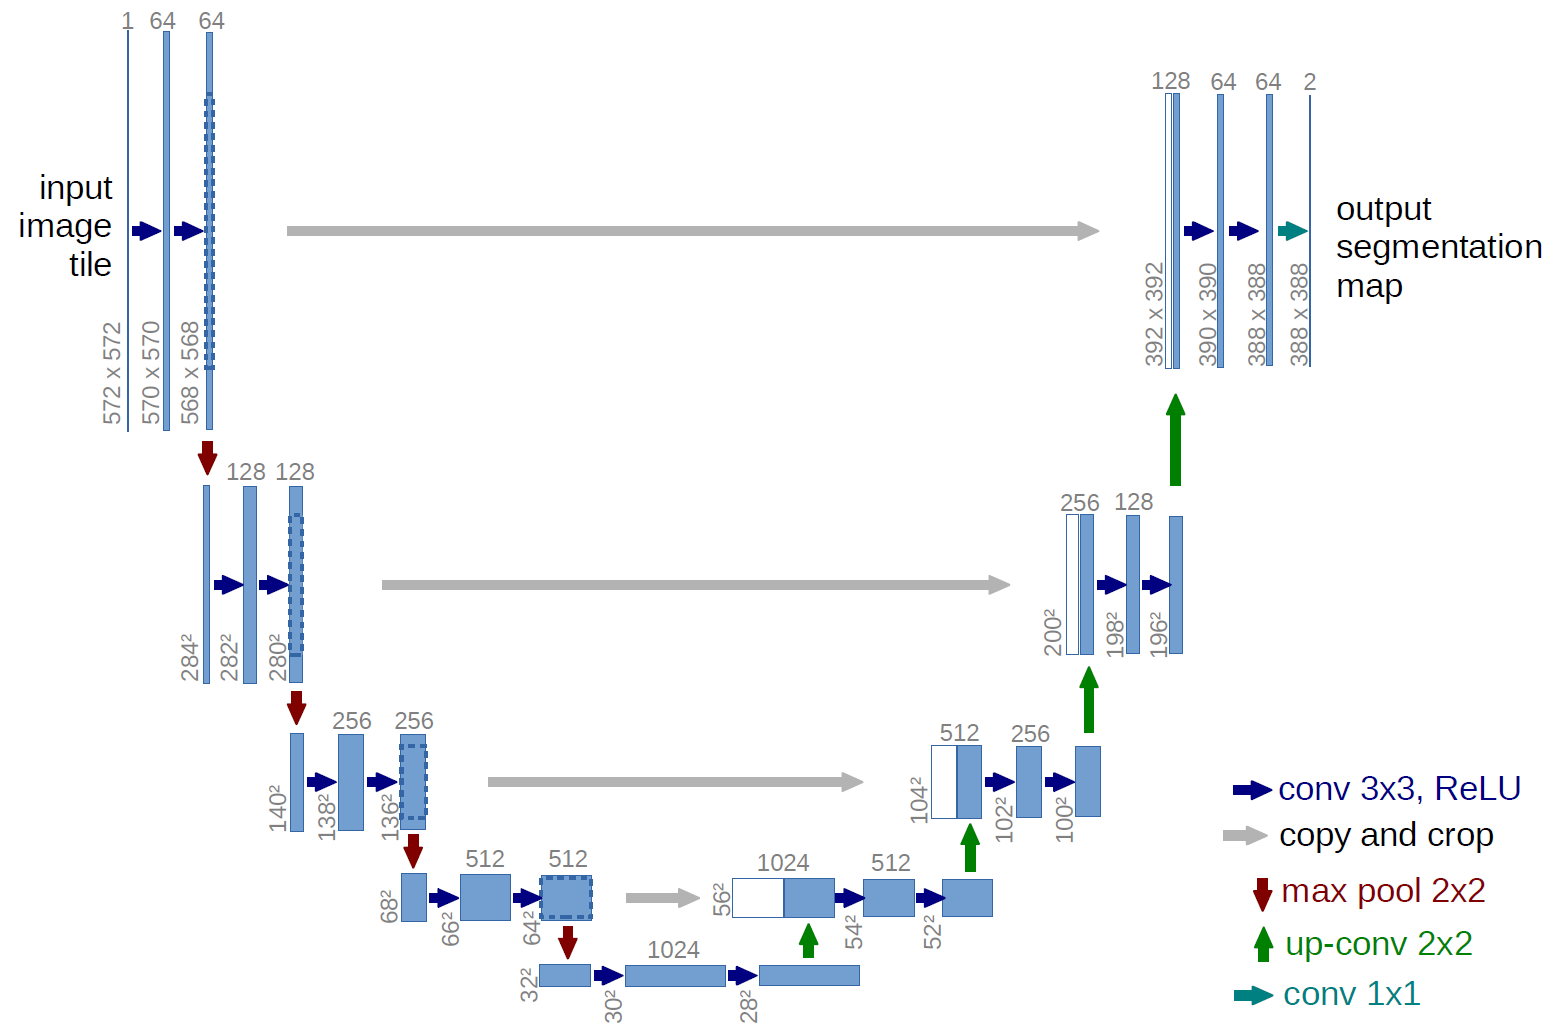
\includegraphics[width=0.99\textwidth]{data/images/u-net-architecture.png}
\caption{Иллюстрация архитектуры U-net из оригинальной статьи \cite{6}}
\label{unet_arch}
\end{figure}

Сеть была названа таким образом из-за U-образной формы. Часть от входа до самого узкого слоя посередине называется кодировщик(encoder), она служит для сжатия входного изображения и извлечения из него самых существенных для решаемой задачи признаков. 
Часть от середины и до выхода называется декодировщик(decoder), она служит для восстановления основной информации исходного изображения(задачу сегментации можно интерпретировать как удаление шума из исходного изображения).

В архитектуру \cite{6} были внесены незначительные изменения:
\begin{itemize}
	\item[--] Уменьшено количество свёрточных фильтров (с 64 до 32).
	
	\item[--] Добавлено заполнение по краям свёрток(padding).
	
	\item[--] Изменена функция активации(с ReLU на ELU).
\end{itemize}

Сеть представляет из себя композицию следующий слоёв: 
\begin{itemize}
	\item[--] Линейных сверток (\ref{conv}):
	
\begin{equation} \label{conv}
\begin{aligned}
	& y_{c, i, j}(x|w) = \sum \limits_{l=1}^{C} 
		\sum \limits_{m=1}^{min(W - i, K)}
		\sum \limits_{n=1}^{min(H - j, K)} 
		x_{l, i + m, j + n} \ w^c_{l, m, n} \\
	& ,\ c = \overline{1, T} 
		,\ i = \overline{1, W}
		,\ j = \overline{1, H} \\
	& \text{, где $x \in \mathbb{R}^{C \times W \times H}$
		- вход свёртки} \\
	& \text{, $y \in \mathbb{R}^{T \times W \times H}$ 
		- выход свёртки} \\
	& \text{, $w^c \in \mathbb{R}^{C \times K \times K}$
		- фильтры свёрток} \\
	& \text{, $c=\overline{1, C}$ - количество свёрток}.
\end{aligned}
\end{equation}

 	\item[--] Объединений выходов слоёв (concatenation, \ref{concat}):
 
\begin{equation} \label{concat}
\begin{aligned}
	& z_{c, i, j}(x, y) = \begin{cases}
		& x_{c, i, j} \text{, если $c \leq C$,} \\
		& y_{c - C, i, j} \text{, если $c > C$}
	\end{cases} \\
	& \text{, где $x \in \mathbb{R}^{C \times W \times H}$
	,\ $y \in \mathbb{R}^{T \times W \times H}$ 
	,\ $z \in \mathbb{R}^{(T + C) \times W \times H}$}
\end{aligned}
\end{equation}

 	\item[--] "Обратных" свёрток(transposed convolution, действие которых эквивалентно обратному действию свёрточных слоев, т.е по выходу свёрточного слоя $y$ и фильтрам $w$ получается вход свёрточного слоя $x$).
 	
 	\item[--] Нелинейных преобразований
активации (\ref{ELU}), (\ref{softmax}), pooling (\ref{pooling}).

\begin{equation} \label{ELU}
	y(x) = \begin{cases} 
		& x ,\ \text{при $x \geq 0$}, \\	
		& e^x - 1 ,\ \text{при $x < 0$}.
	\end{cases}
\end{equation}

\begin{equation} \label{softmax}
\begin{aligned}
	& y_{c, i, j}(x) = \frac{ e^{x_{c, i, j}} }
		{ \sum \limits_{l=1}^{C} e^{x_{l, i, j}} } \\
	& x \in \mathbb{R}^{C \times W \times H}
		,\ y \in \mathbb{R}^{C \times W \times H}
\end{aligned}
\end{equation}

\begin{equation} \label{pooling}
\begin{aligned}
	y_{c, i, j}(x) & = \max \limits_{
		\substack{
			m=\overline{1, min(W - i, K)}
			\\ n=\overline{1, min(H - j, K)}}}
		x_{c, i K + m, j K + n} \\
	& \text{, где $x \in \mathbb{R}^{C \times W \times H}$ 
		- вход pooling'а} \\
	& \text{, $y \in \mathbb{R}
		^{C 
		  \times \bigl[ \frac{W + K - 1}{K} \bigr] 
		  \times \bigl[ \frac{H + K - 1}{K} \bigr] }$ 
		- выход pooling'а} \\
	& \text{, $K$ - размер ядра pooling'а}.
\end{aligned}
\end{equation}

	\item[--] Слоя выпадения сигнала(dropout (\ref{dropout})).

\begin{equation} \label{dropout}
\begin{aligned}
	&y(x) = D \odot x, \text{ где
		$x \in \mathbb{R}^{C \times W \times H},\ 
		D = (d_{kijk})_{k=1,i=1,j=1}^{C, W, H},\ d_{ijk} \sim B(p)$}
\end{aligned}
\end{equation}

\end{itemize}
	
Данные преобразования применяются последовательно, порядок композиции показан на рис.\ref{unet_arch}. 
Количество pooling(\ref{pooling}), concatetation(\ref{concat}) и
transposed convolution слоёв подобрано так, чтобы выходной тензов имел такие же пространственные размерности $H \times W$, что и входной, и 2 канала(вместо одного на входе). Для улучшения обобщающей способности сети и предотвращению переобучения на стыке кодировщика и декодиковщика расположен слой (\ref{dropout}). Вероятности на выходе обеспечиваются с помощью 
softmax-преобразования выхода сети (\ref{softmax}). 

В итоге модель реализует следующее отображение: 
\begin{equation} \label{model}
\begin{aligned}
	& f_{\theta}(x) = y, \\
	& x \in \mathbb{R}^{1 \times H \times W}
		,\ y \in 
		\mathbb{R}^{2 \times H \times W}
\end{aligned}
\end{equation}

, где первая первая размерность -- число каналов изображения(на входе один, потому что изображение grayscale; на выходе два: в первом канале вероятность того, что текущий пиксель -- это пора, во втором -- что это твёрдое вещество), последние две размерности -- это размер изображений. В качестве оптимизируемых в задаче (\ref{opt}) параметров модели $\theta$ выступает совокупность весов convolutional и transposed convolutional слоёв.

\clearpage

\newpage


\section{Оптимизация модели} \label{seg_optimization}

В данной главе даётся законченная формулировка задачи (\ref{opt}), вводится конкретная функция потерь. Указывается метод оптимизации для решения поставленной задачи с конкретной моделью из предыдущей главы.

\subsection{Оптимизируемый функционал}

Для финальной постановки задачи осталось выбрать функцию потерь 
$\mathcal{L}(\overline{Y}, Y)$. Поскольку выход модели (\ref{model})
является бинарными вероятностями, подходящей функцией является кросс-энтропия:
\begin{equation} \label{cross-entropy}
	CE(\overline{Y}, Y) = -\frac{1}{W H} \sum \limits_{i=1, j=1}^{W, H} \Bigl(
		Y_{ij} \log \overline{Y}_{0ij} 
		+ (1 - Y_{ij}) \log (1 - \overline{Y}_{1ij}) \Bigr).
\end{equation}

Выбор обуславливается тем, что функция  \ref{cross-entropy} гладкая, выпуклая, минимум достигается 
при выборе с помощью прогноза $\overline{Y}$ верного класса, и она
имеет понятную и адекватную вероятностную интерпретацию.

Так же в качестве метрики качества в задачах сегментации используют коэффициент Жаккара: 
\begin{equation} \label{jaccard}
	J(A, B) = \frac{|A \cap B|}{|A \cup B|} 
\end{equation}
, где в качестве множеств $A$ и $B$ выступают множество пикселей, отнесённые к 
первому(второму) классу моделью, и множество пикселей, образующих правильный ответ для первого(второго) класса.

Коэффициент Жакарра (\ref{jaccard}) нельзя использовать для обучения модели напрямую, потому что для его вычисления требуется определённый(метка конкретного класса) прогноз модели, а модель 
(\ref{model}) возвращает вероятности меток. При переходе от вероятности к меткам по порогу(например, при $p< \tau=0.5$ предсказывается первый класс, иначе -- второй) функция перестаёт быть гладкой:

\begin{equation} \label{threshold}
	y(x) = \begin{cases} 
		& 0 ,\ \text{при $x \leq \tau$}, \\	
		& 1 ,\ \text{при $x > \tau$}.
	\end{cases}
\end{equation}

Поэтому в качестве функции потерь можно использовать гладкую аппроксимацию (\ref{jaccard}). Можно придумать различные виды аппроксимации, в данной работе применялась следующая(такой подход использован в \cite{20}):
\begin{equation} \label{smoothed_iou}
	sIOU(\overline{Y}, Y) = \frac{1}{W H}
		\sum \limits_{i=1, j=1}^{W, H}
		\frac{Y_{ij} \overline{Y}_{ij} + \varepsilon}
		{Y_{ij} + \overline{Y}_{ij} 
			- Y_{ij} \overline{Y}_{ij} + \varepsilon}.
\end{equation} 
 
Можно убедиться, что при ''стремлении'' 
$\overline{Y}$ к $Y$ значение $sIOU(\overline{Y}, Y)$ стремится к $J(A(\overline{Y}, \tau), Y)$ при любом выборе порога $\tau$. В выражении (\ref{smoothed_iou}) фигурирует 
константа $\varepsilon$(на практике, например, $\varepsilon=10^{-5}$), которая используется для вычислительной стабильности.
 
Итоговая фунция потерь, которая использовалась для оптимизации модели, имеет вид:
\begin{equation} \label{final_loss}
	\mathcal{L}(\overline{Y}, Y) = CE(\overline{Y}, Y)
		- \gamma \log \bigl( sIOU(\overline{Y}, Y) \bigr)
\end{equation}
, где $\gamma$ - коэффициент соотношения функций потерь. Величина (\ref{smoothed_iou}) находится под логарифмом для коррекции соотношения к величине (\ref{cross-entropy}). Аппроксимация для индекса Жакарра взята с отрицательным знаком потому, что при увеличении качества модели значение индекса увеличивается.

\subsection{Метод оптимизации}

Последним шагом для завершения модели является выбор метода решения 
задачи (\ref{model}) для функции потерь (\ref{final_loss}).

Для задач оптимизации параметров нейронных сетей характерны следующие особенности:
\begin{itemize}
	\item Большое число оптимизируемых параметров.
	
	\item Непрерывное пространство оптимизируемых параметров.
	
	\item Возможность аналитического вычисления градиентов с помощью
алгоритма обратрого распространения ошибок(back propogation).
		
	\item Сложная структура оптимизируемого функционала: отсутствие 	выпуклости, множество седловых точек и локальных минимумов.
	
	\item Большой размер обучающей выборки.
	
\end{itemize} 
	
В связи с непрерывной структурой пространства параметров и возможностью вычислять аналитические градиенты, эвристические(отжиг, генетические алгоритмы) методы для оптимизации параметров нейронных сетей применяются редко. Из-за огромного числа параметров квадратичные методы оптимизации не применимы. Квазиньютовоские методы тоже, как правило, оказываются неоправданно медленными. Для обучения используются тренировочные выборки большого размера, поэтому методы оптимизации должны обрабатывать выборку порционно(по батчам). 

По этим причинам задачи оптимизации в нейронных сетях решаются в основном с помощью вариаций стохастического градиента. В основном используются варианты с моментумом(для выхода из седловых точек и плохих локальных минимумов) и адаптивным темпом обучения. В данной работе в качестве метода оптимизации использовался ADAM \cite{19}.

\newpage


\section{Ход работы} \label{seg_tasks}

\subsection{Прикладная задача}

Задача, которая стояла перед началом работы, -- проверить возможность применения глубинного обучения для сегментации изображений геологических пород. 
Методы глубинного обучения выглядят привлекательными для данной задачи по следующим причинам:
\begin{itemize}
	\item Автоматическая оптимизации параметров, а значит полной 	независимости от оператора.
	
	\item Оптимизация на этапе обучения, отсутствие оптимизации на этапе прогноза.
	
	\item Высокая обобщающая способность, возможность построения универсальной модели для широкого класса пород.
	
\end{itemize}
 
\subsection{Данные для экспериментов}

Из-за наличия обучения возникает проблема формирования обучающей выборки: сейчас не существует коллекции правильно размеченных томограмм геологических пород. Альтернативой является использование в качестве обучающей выборки изображений, полученных с помощью других, необучаемых и эталонных методов под контролем оператора. Именно такой путь был выбран в данной работе.

\begin{table}[h!]
\caption{Сравнение количественных данных по влиянию искажений на результат декодирования}
\begin{center}
\begin{tabular}{|c|c|c|c|}
\hline
\multicolumn{4}{|c|}{\textbf{Образцы пород}}\\
\hline
\textbf{Тип} & \textbf{Название} & \textbf{Размеры} 
	& \textbf{Разрешение} \\ \hline
\multirow{4}{*}{Карбонаты} & carb96558 & $720^3$ & $5.39 \mu m$ \\ 
& carb71 & $720^3$ & $2.63 \mu m$ \\ 
& carbRNF & $700^3$ & $2.24 \mu m$ \\ 
& SPE-carb & $509^3$ & $ 5.75 \mu m$ \\ \hline
\multirow{4}{*}{Почвы} & SoilAh-1 & $700^3$ & $20.96 \mu m$ \\ 
& SoilB-2 & $700^3$ & $16.19 \mu m$ \\ 
& TiTree-1 & $710^3$ & $ 5.24 \mu m$ \\ 
& TiTree-2 & $710^3$ & $ 5.24 \mu m$ \\ \hline
\multirow{3}{*}{Песчаники} & Urna-22 & $710^3$ & $5.17 \mu m$ \\ 
& Urna-30 & $710^3$ & $4.86 \mu m$ \\ 
& Urna-34 & $700^3$ & $4.71 \mu m$ \\ \hline
\end{tabular}
\end{center}
\caption{Характеристика используемых образцов}
\label{samples}
\end{table}

В качестве тренировочной выборки были выбраны образцы следующих пород(таб. \ref{samples}): карбонаты(4 образца, названия: carb96558, carb71, carbRNF, SPE-carb)  почвы(4 образца, названия: SoilAh-1, SoilB-2, TiTree-1, TiTree-2) и песчаники(3 образца, названия: Urna-22, Urna-30, Urna-34). Образцы специально подбирались достаточно разнородными, отличаются породы, размеры и разрешение использовавшегося томографа.

В	качестве истинной сегментации использовались изображения, полученные с помощью метода CAC(convergene active contours) \cite{12}.


\subsection{Разделение данных на обучающие и тестовые}

В ходе работы было построено 7 молелей, каждая модель использовала 700 пар изображение-сегментация, размеры изображений соответствуют размерам в таб. \ref{samples}.

Модели можно разделить на три группы:
\begin{enumerate}
	\item Одиночные модели:
	\begin{itemize}
		\item Модель для карбонатов обучалась на образце carb96558.
	
		\item Модель для почв обучалась на образце SoilB-2.
	
		\item Модель для песчаников обучалась на образце Urna-22.
	\end{itemize}
	
	\item Парные модели:
	\begin{itemize}	
		\item Парная модель для карбонатов и почв обучалась на образцах carb96558 и SoilB-2, обучающие пары распрелелялись в пропорции $1:1$.
	
		\item Парная модель для карбонатов и песчаников обучалась на образцах carb96558 и Urna-22, обучающие пары распрелелялись в пропорции $1:1$.
	
	\item  Парная модель для песчаников и почв обучалась на образцах Urna-22 и SoilB-2, обучающие пары распрелелялись в пропорции $1:1$
	\end{itemize}
	
	\item  Общая модель для песчаников, почв и карбонатов обучалась на образцах Urna-22, SoilB-2 и carb96558, обучающие пары распрелелялись в пропорции $1:1:1$.
	
\end{enumerate}


\newpage


\section{Результаты} \label{seg_results}

\subsection{Обучение моделей}

Процесс обучения состоял из 10 эпох. В каждой эпохе модель обучалась на случайной подвыборке тренировочной выборки, размер случайной подвыборки $\frac{1}{5}$ от всей выборки. Таким образом каждый обучающий пример подавался в модель в среднем 2 раза за время обучения. В качестве входных данных модели подавались 2-D фрагменты изображений образцов размером $64 \times 64$, которые были получены разделением исходных изображений на части с минимальным наложением.
Все изображения образца расположены в одной плоскости, 3-D структура образца формируется путём ''наложения'' изображений друг на друга.

В качестве целевого функционала использовался (\ref{final_loss}) с 
$\gamma=1, \varepsilon=10^{-5}$. Модель обучалась с помощью метода 
ADAM \cite{19} с параметрами \\
$\alpha=10^{-3}, \beta_1=0.9, \beta_2=0.999$. Так же использовалось 
мультипликативное понижение темпа обучение, т.е. на каждой эпохе 
$\alpha$ домножалось на темп снижения $\lambda=\sqrt[10]{10^{-2}}$( такая константа выбрана для того, чтобы на последней эпохе темп обучения снизился до $\alpha=10^{-5}$).

В процессе обучения отслеживалась величина оптимизируемого функционада (\ref{final_loss}), а так же следующие функции качества:
logistic loss (\ref{cross-entropy}), sIOU (\ref{smoothed_iou}) и 
точность предсказаний по фиксированному порогу $\tau=0.5$. 

\begin{figure}[h!]
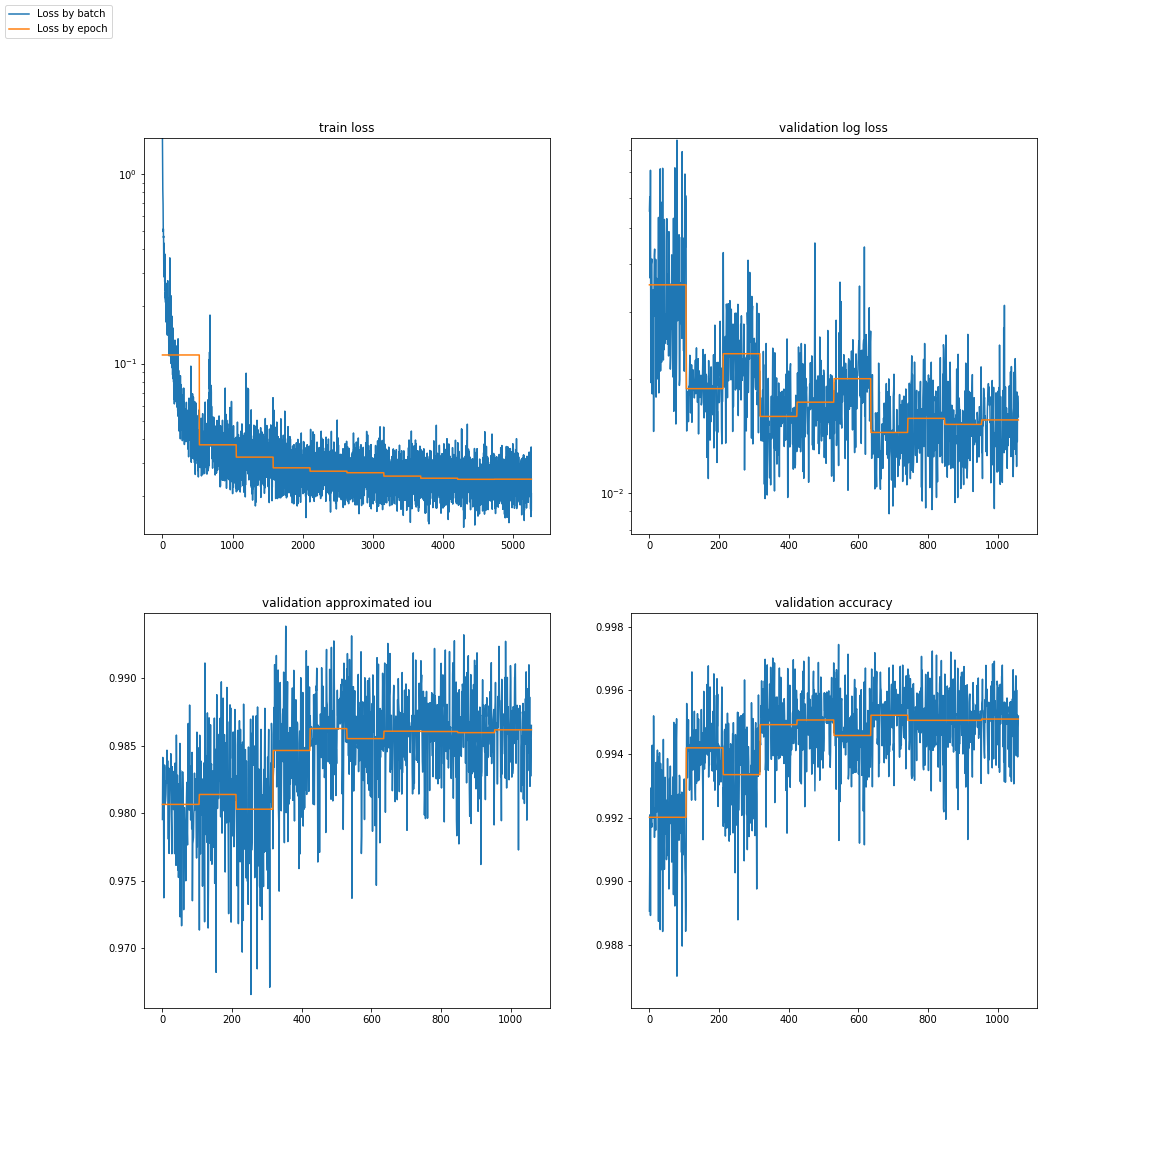
\includegraphics[width=0.99\textwidth]{data/images/learning_progress_SoilB-2.png}
\caption{График кривой обучения для одиночной модели из группы 1, обученной на образце SoilB-2.}
\label{learning1}
\end{figure}

\begin{figure}[h!]
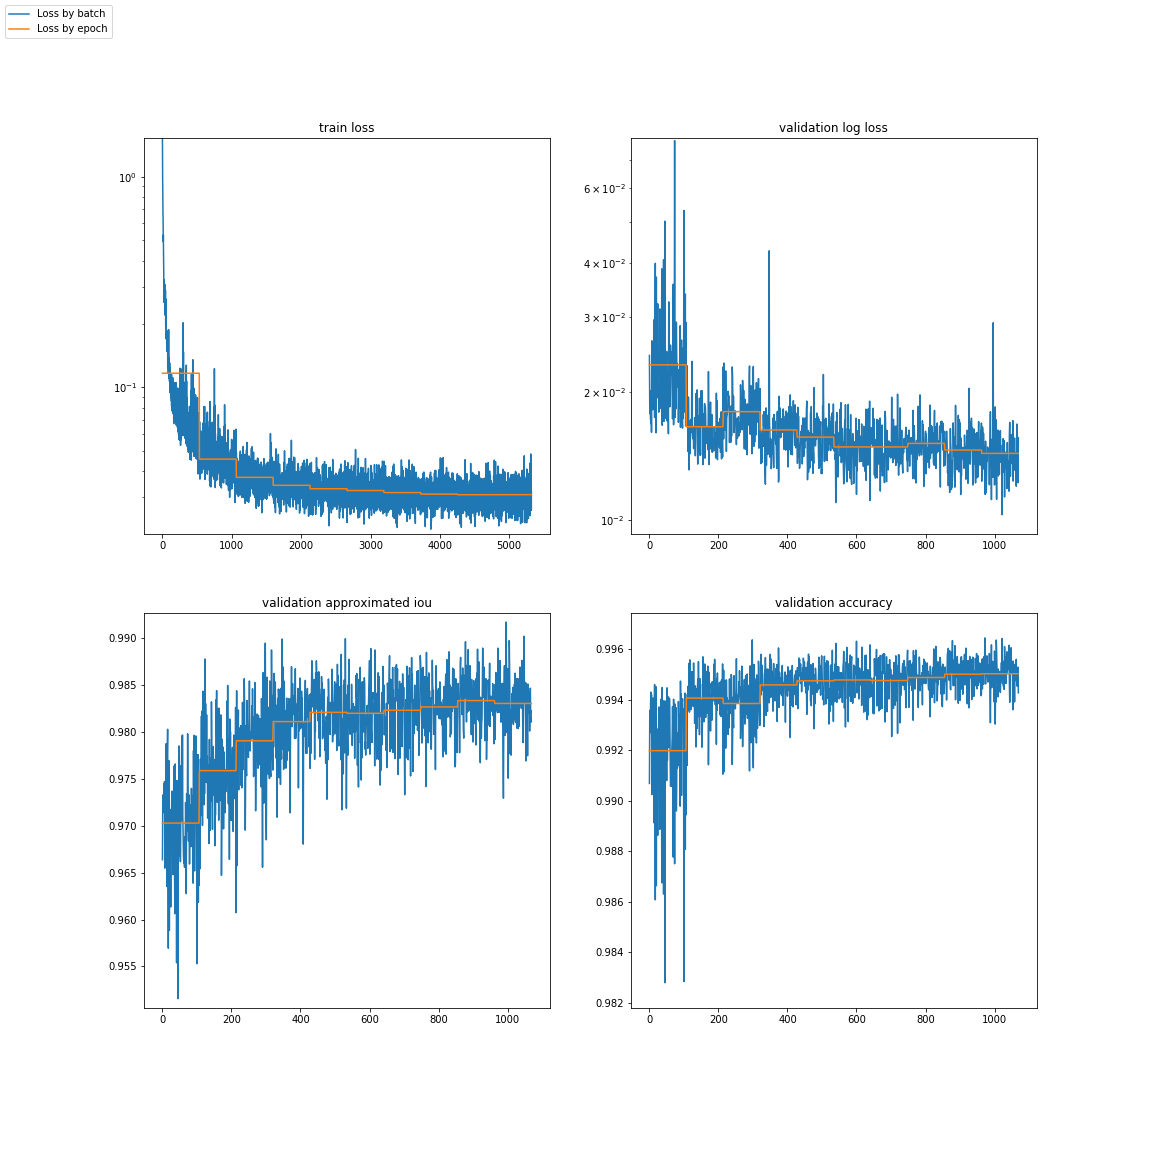
\includegraphics[width=0.99\textwidth]{data/images/learning_progress_SoilB-2_Urna_22_carb96558.png}
\caption{График кривой обучения для общей модели группы 3.}
\label{learning2}
\end{figure}

На рис. \ref{learning1}, \ref{learning2} приведены примеры кривой обучения для нескольких моделей. Видно, что метрики ведут себя согласованно(т.е. сохраняется тренд повышения качества по всем метрикам). К последним эпохам метрики выходят на плато, что говорит о стабилизации параметров модели.

\subsection{Выбор порога вероятности} 

В рамках прикладной задачи по обработке образцов томограмм геологических пород от модели требуется получение бинарной маски предсказанных классов для пикселей исходного изображения. Модель 
(\ref{model}) предоставляет распределение вероятностей классов. Для того, чтобы перейти от вероятностей к бинарным меткам, треуется выбрать порог перехода $\tau$(для отслеживания прогресса в обучении модели, как указано в предыдущем порразделе, выбиралось $\tau=0.5$) для функции (\ref{threshold}).
Поскольку конечная цель данной работы - это получение модели с высокой обобщающей способностью, применимой к различным видам пород, подбор параметра порога $\tau$ выглядит затруднительной задачей(в самом деле, он может быть разным для разных образцов пород, а значит его нельзя заранее получить для образцов, которые обрабатываются впервые, и для которого нет аналогичных обработанных образцов).

В ходе экспериментов было установлено, что 
модель (\ref{model}), которая тренируется для минимизации функции качества (\ref{final_loss}), имеет необычную(нехарактерную для подобных моделей) плотность распределения вероятностей пикселей $f(p)$ - вся вероятностая масса расположена вблизи 0 и 1. Это значит, что качество бинарного прогноза модели устойчиво к выбору порога в широком интервале(в эксперимента любой порог $\tau \in [0.1,\ 0.9]$ показывал примерно аналогичный результат, иллюстрация на рис. \ref{threshold_p}). Из вышесказанного следует, что данное свойство модели имеет большое практическое значение. 

\begin{figure}[h!]
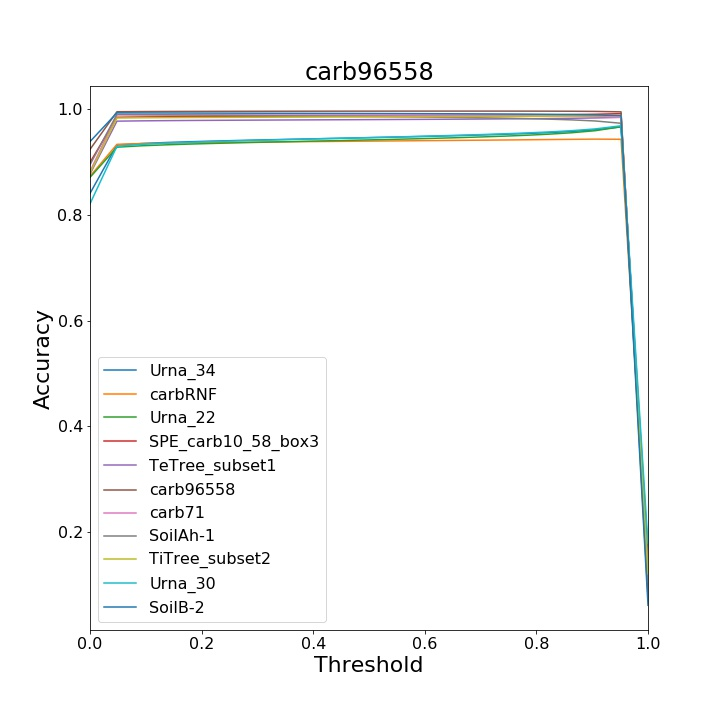
\includegraphics[width=0.9\textwidth]{data/images/accuracy.jpg}
\caption{Зависимость точности предсказания от величины порога вероятности $\tau$ для модели из группы 1, обученной на образце carb96558.}
\label{threshold_p}
\end{figure}

\subsection{Оценка ошибок в разных плоскостях} \label{planes}

Поскольку обучающие примеры были взяты из одной плоскости, а образцы являются трёхмерными, требовалось проверить качество предсказания модели в другой плоскости, ортогональной плоскости, из которой брались обучающие примеры. 

Эксперименты показали, что нет существенного различия в качестве сегментации для изображений, взятых из различных плоскостей, имеет место равентсво функционалов качества, а так же визуальная эквивалентность результатов. 

Примеры полученных результатов на рис. \ref{res_all}, \ref{res_soil_urna}. Зелёным цветом показанны правильно предсказанные моделью поры, красным -- неправильно предсказанные моделью поры, синим -- неправильно предсказанное моделью твёрдое вещество. Видно, что предсказание модели и правильный ответ для изображений почти не различается.

\begin{figure}[h!]
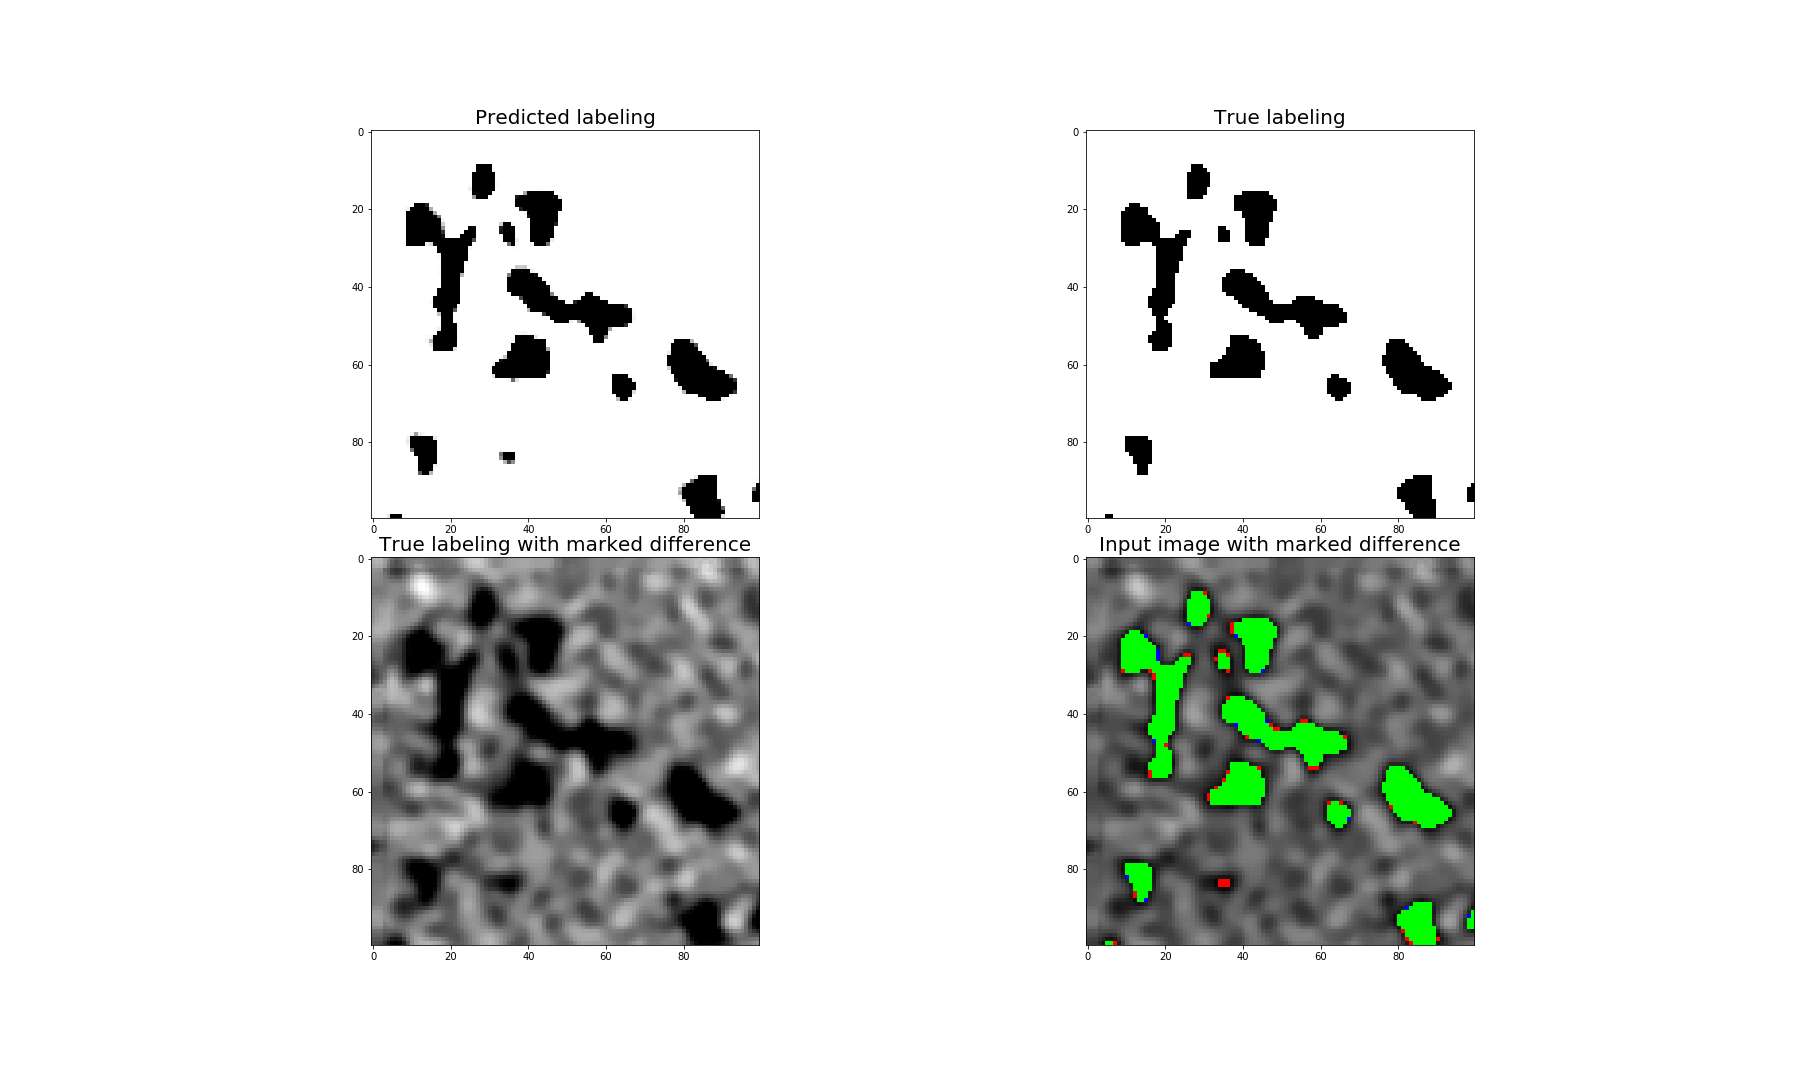
\includegraphics[width=0.99\textwidth]{data/images/all_carb71.png}
\caption{Результаты модели из группы 3 на образце carb71.}
\label{res_all}
\end{figure}


\begin{figure}[h!]
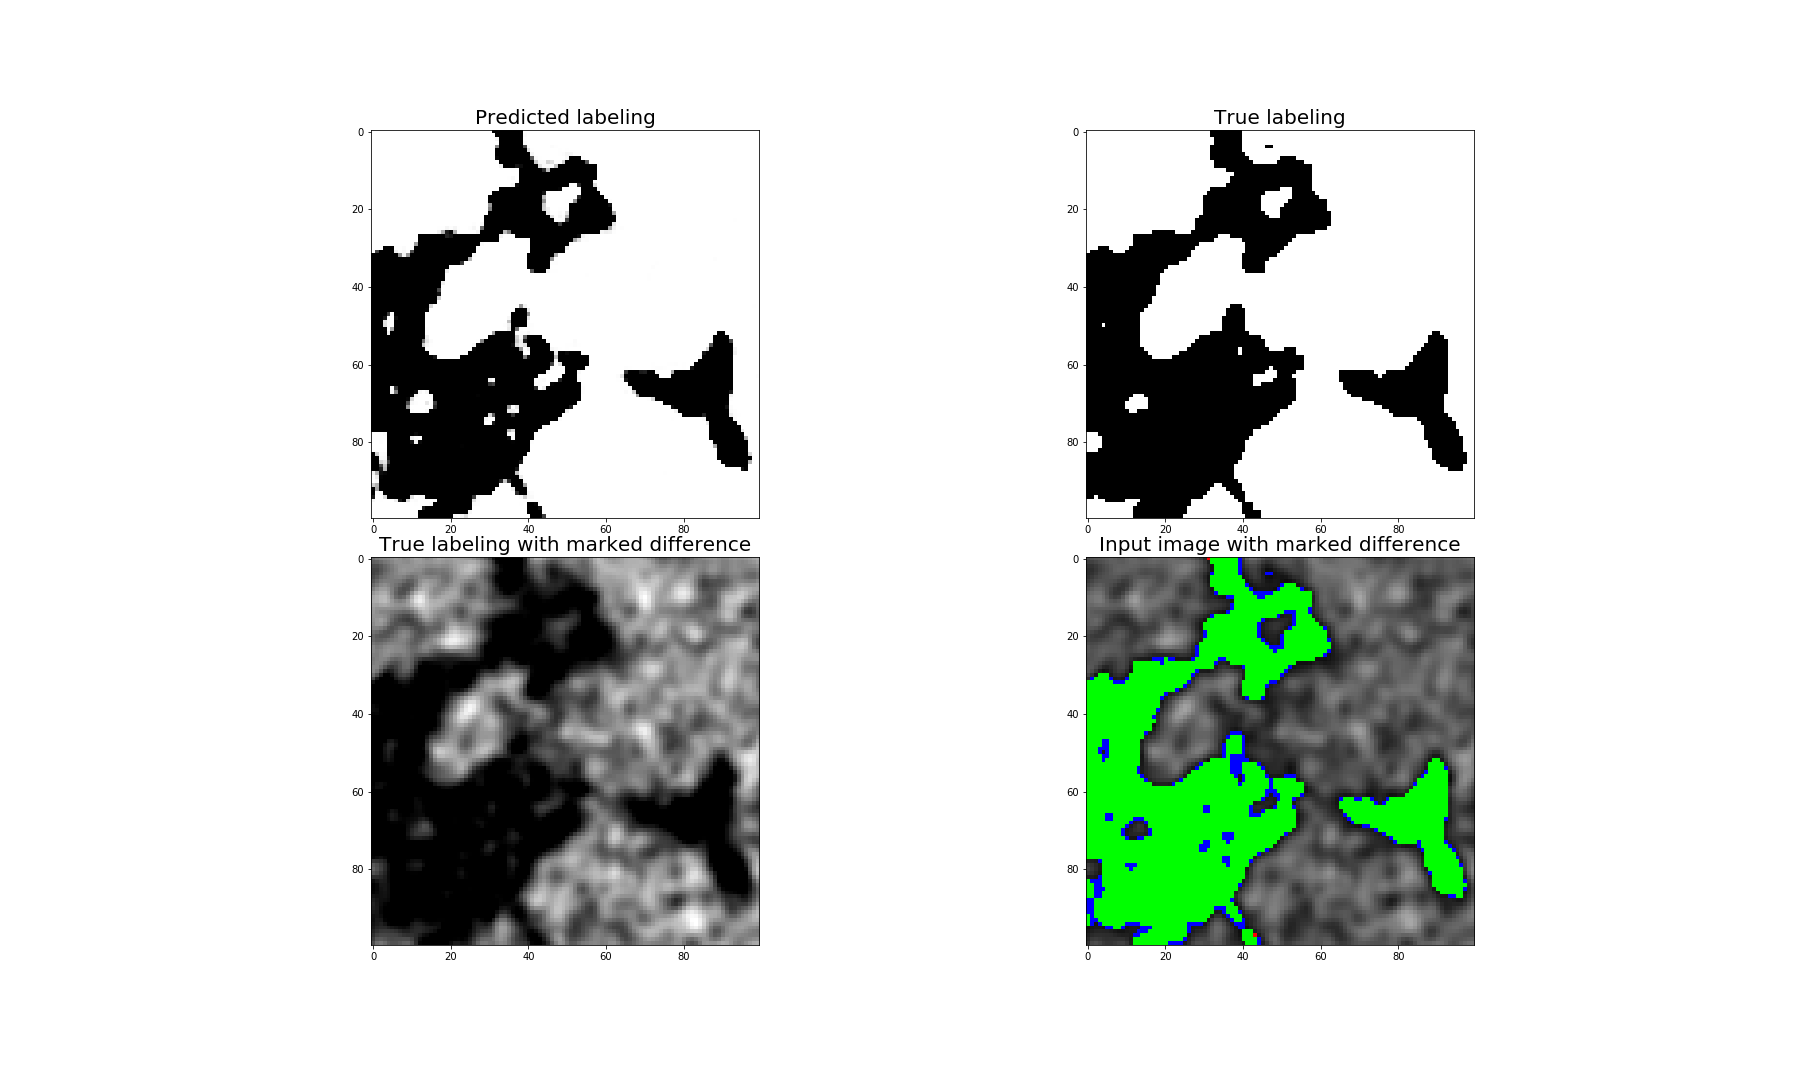
\includegraphics[width=0.99\textwidth]{data/images/Soil_Urna_SPE_carb10_58_box3.png}
\caption{Результаты модели из группы 2, обученной на образцах Urna-22 и SoilB-2, на образце SPE-carb.}
\label{res_soil_urna}
\end{figure}

\subsection{Оценка качества моделей}

Для оценки качества моделей использовались следующие метрики:
\begin{itemize}
	\item[--] logloss (\ref{cross-entropy}),
	
	\item[--] IOU (\ref{jaccard}),
	
	\item[--] precision -- точность предсказания(отношение истинно предсказанных меток первого класса к общему числу предсказанных меток первого класса),
	
	\item[--] recall -- полнота предсказания(отношение истинно предсказанных меток первого класса к общему числу правильных меток первого класса),
	
	\item[--] PR-AUC -- площадь под кривой зависимости точности от полноты, 
	
	\item[--] accuracy -- верность предсказания (число правильно предсказанных меток первого и второго класса к общему числу пикселей).
\end{itemize}

Результаты для обученных меделей приведены в таблицах \ref{carb96558}-\ref{Urna_34}. Таблицы организованны следующим образом: каждая таблица показывает результат работы всех моделей на данном образце, выделенные значения -- лучший результат конкретной метрики среди всех моделей. 

Результаты можно охарактеризовать следующим образом:
\begin{itemize}
	\item Модели из группы 1 хорошо работают для образцов того типа, на котором были обучены, на остальных образцах результаты заметно хуже.
	
	\item Модели из групп 2-3 работают хорошо на большинстве образцов, но хуже, чем модели из 1 на специфичных для них образцах.
	
	\item Образцы в почвах похожи на песчаники, поэтому модели, обученные на песчаниках, хорошо отрабатывают для почв(в обратную сторону связь не действует, песчаники более специфичной структуры).
	
	\item Есть специфичные образцы, на которых большинство моделей работают не лучшим образом(carbRNF), они специально были добавлены для проверки результатов. На этом образце лучше всего работает модель из группы 1 для песчаников, что объясняет специфичность данного образца(карбонат, но похож на песчаник).
	
	\item Модель из группы 3 показывает себя относительно хорошо на всех образцах.
	
\end{itemize}

\begin{table}[htbp]
\small
\begin{tabular}{|c|r|r|r|r|r|r|}
\hline
\textbf{Модель} & \multicolumn{ 6}{c|}{\textbf{Метрика}} \\ \hline
\textbf{} & \multicolumn{1}{c|}{\textbf{logloss}} & \multicolumn{1}{c|}{\textbf{PR-AUC}} & \multicolumn{1}{c|}{\textbf{iou}} & \multicolumn{1}{c|}{\textbf{accuracy}} & \multicolumn{1}{c|}{\textbf{precision}} & \multicolumn{1}{c|}{\textbf{recall}} \\ \hline
\textbf{carb96558} & 0,0626 & 0,9999 & \textbf{0,9883} & \textbf{0,9897} & 0,9948 & 0,9935 \\ \hline
\textbf{SoilB-2} & 0,0856 & 0,9993 & 0,9719 & 0,9747 & 0,9768 & 0,9949 \\ \hline
\textbf{Urna-22} & 0,2514 & 0,9992 & 0,9740 & 0,9771 & \textbf{0,9996} & 0,9744 \\ \hline
\textbf{Carb96558 + SoilB-2} & \textbf{0,0421} & \textbf{0,9999} & 0,9882 & 0,9895 & 0,9917 & \textbf{0,9965} \\ \hline
\textbf{Carb96558 + Urna\_22} & 0,1248 & 0,9997 & 0,9847 & 0,9865 & 0,9977 & 0,9870 \\ \hline
\textbf{SoilB-2 + Urna-22} & 0,0982 & 0,9998 & 0,9863 & 0,9879 & 0,9977 & 0,9886 \\ \hline
\textbf{All} & 0,0842 & 0,9999 & 0,9872 & 0,9887 & 0,9974 & 0,9897 \\ \hline
\end{tabular}
\caption{Результаты для образца carb96558.}
\label{carb96558}
\end{table}


\begin{table}[htbp]
\small
\begin{tabular}{|c|r|r|r|r|r|r|}
\hline
\textbf{Модель} & \multicolumn{ 6}{c|}{\textbf{Метрика}} \\ \hline
\textbf{} & \multicolumn{1}{c|}{\textbf{logloss}} & \multicolumn{1}{c|}{\textbf{PR-AUC}} & \multicolumn{1}{c|}{\textbf{iou}} & \multicolumn{1}{c|}{\textbf{accuracy}} & \multicolumn{1}{c|}{\textbf{precision}} & \multicolumn{1}{c|}{\textbf{recall}} \\ \hline
\textbf{carb96558} & 0,2977 & 0,9907 & 0,9317 & 0,9361 & 0,9336 & \textbf{0,9978} \\ \hline
\textbf{SoilB-2} & 1,2784 & 0,9030 & 0,8311 & 0,8346 & 0,8848 & 0,9320 \\ \hline
\textbf{Urna-22} & \textbf{0,1345} & \textbf{0,9994} & \textbf{0,9727} & \textbf{0,9760} & \textbf{0,9921} & 0,9803 \\ \hline
\textbf{Carb96558 + SoilB-2} & 0,6819 & 0,9274 & 0,8992 & 0,9033 & 0,9098 & 0,9872 \\ \hline
\textbf{Carb96558 + Urna-22} & 0,1551 & 0,9968 & 0,9598 & 0,9637 & 0,9664 & 0,9929 \\ \hline
\textbf{SoilB-2 + Urna-22} & 0,3964 & 0,9935 & 0,9223 & 0,9292 & 0,9568 & 0,9624 \\ \hline
\textbf{All} & 0,2835 & 0,9890 & 0,9380 & 0,9429 & 0,9474 & 0,9895 \\ \hline
\end{tabular}
\caption{Результаты для образца carbRNF.}
\label{carbRNF}
\end{table}

\begin{table}[htbp]
\small
\begin{tabular}{|c|r|r|r|r|r|r|}
\hline
\textbf{Модель} & \multicolumn{ 6}{c|}{\textbf{Метрика}} \\ \hline
\textbf{} & \multicolumn{1}{c|}{\textbf{logloss}} & \multicolumn{1}{c|}{\textbf{PR-AUC}} & \multicolumn{1}{c|}{\textbf{iou}} & \multicolumn{1}{c|}{\textbf{accuracy}} & \multicolumn{1}{c|}{\textbf{precision}} & \multicolumn{1}{c|}{\textbf{recall}} \\ \hline
\textbf{carb96558} & 0,0473 & \textbf{0,9999} & 0,9848 & 0,9861 & 0,9848 & 1,0000 \\ \hline
\textbf{SoilB-2} & 0,0695 & 0,9998 & 0,9789 & 0,9806 & 0,9790 & 0,9999 \\ \hline
\textbf{Urna-22} & 0,0668 & 0,9999 & \textbf{0,9900} & \textbf{0,9910} & \textbf{0,9966} & 0,9934 \\ \hline
\textbf{Carb96558 + SoilB-2} & 0,0590 & 0,9999 & 0,9827 & 0,9841 & 0,9827 & \textbf{1,0000} \\ \hline
\textbf{Carb96558 + Urna-22} & 0,0500 & 0,9990 & 0,9879 & 0,9890 & 0,9883 & 0,9996 \\ \hline
\textbf{SoilB-2 + Urna-22} & 0,0379 & 0,9998 & 0,9874 & 0,9886 & 0,9876 & 0,9999 \\ \hline
\textbf{All} & \textbf{0,0353} & 0,9998 & 0,9869 & 0,9881 & 0,9870 & 0,9999 \\ \hline
\end{tabular}
\caption{Результаты для образца SPE-carb.}
\label{SPE_carb}
\end{table}


\begin{table}[htbp]
\small
\begin{tabular}{|c|r|r|r|r|r|r|}
\hline
\textbf{Модель} & \multicolumn{ 6}{c|}{\textbf{Метрика}} \\ \hline
\textbf{} & \multicolumn{1}{c|}{\textbf{logloss}} & \multicolumn{1}{c|}{\textbf{PR-AUC}} & \multicolumn{1}{c|}{\textbf{iou}} & \multicolumn{1}{c|}{\textbf{accuracy}} & \multicolumn{1}{c|}{\textbf{precision}} & \multicolumn{1}{c|}{\textbf{recall}} \\ \hline
\textbf{carb96558} & 0,0666 & 0,9999 & 0,9886 & 0,9898 & 0,9980 & 0,9906 \\ \hline
\textbf{SoilB-2} & 0,0349 & 0,9999 & 0,9873 & 0,9885 & 0,9904 & 0,9968 \\ \hline
\textbf{Urna-22} & 0,4208 & 0,9994 & 0,9558 & 0,9604 & \textbf{1,0000} & 0,9558 \\ \hline
\textbf{Carb96558 + SoilB-2} & \textbf{0,0342} & 0,9999 & 0,9884 & 0,9895 & 0,9914 & \textbf{0,9969} \\ \hline
\textbf{Carb96558 + Urna-22} & 0,1753 & 0,9999 & 0,9789 & 0,9811 & 0,9998 & 0,9790 \\ \hline
\textbf{SoilB-2 + Urna-22} & 0,0877 & \textbf{0,9999} & 0,9861 & 0,9875 & 0,9993 & 0,9868 \\ \hline
\textbf{All} & 0,0551 & 0,9999 & \textbf{0,9892} & \textbf{0,9903} & 0,9978 & 0,9914 \\ \hline
\end{tabular}
\caption{Результаты для образца SoilAh-1.}
\label{SoilAh-1}
\end{table}

\begin{table}[htbp]
\small
\begin{tabular}{|c|r|r|r|r|r|r|}
\hline
\textbf{Модель} & \multicolumn{ 6}{c|}{\textbf{Метрика}} \\ \hline
\textbf{} & \multicolumn{1}{c|}{\textbf{logloss}} & \multicolumn{1}{c|}{\textbf{PR-AUC}} & \multicolumn{1}{c|}{\textbf{iou}} & \multicolumn{1}{c|}{\textbf{accuracy}} & \multicolumn{1}{c|}{\textbf{precision}} & \multicolumn{1}{c|}{\textbf{recall}} \\ \hline
\textbf{carb96558} & 0,1097 & 0,9995 & 0,9762 & 0,9788 & 0,9819 & 0,9941 \\ \hline
\textbf{SoilB-2} & 0,1414 & 0,9972 & 0,9578 & 0,9615 & 0,9595 & 0,9982 \\ \hline
\textbf{Urna-22} & 0,0728 & 0,9999 & 0,9891 & 0,9904 & \textbf{0,9972} & 0,9919 \\ \hline
\textbf{Carb96558 + SoilB-2} & 0,0786 & 0,9995 & 0,9788 & 0,9810 & 0,9791 & 0,9996 \\ \hline
\textbf{Carb96558 + Urna-22} & 0,0276 & \textbf{0,9999} & \textbf{0,9907} & \textbf{0,9917} & 0,9921 & 0,9986 \\ \hline
\textbf{SoilB-2 + Urna-22} & \textbf{0,0218} & 0,9999 & 0,9904 & 0,9915 & 0,9911 & 0,9993 \\ \hline
\textbf{All} & 0,0268 & 0,9999 & 0,9881 & 0,9895 & 0,9884 & \textbf{0,9997} \\ \hline
\end{tabular}
\caption{Результаты для образца TeTree-1}
\label{TeTree_1}
\end{table}

\begin{table}[htbp]
\small
\begin{tabular}{|c|r|r|r|r|r|r|}
\hline
\textbf{Модель} & \multicolumn{ 6}{c|}{\textbf{Метрика}} \\ \hline
\textbf{} & \multicolumn{1}{c|}{\textbf{logloss}} & \multicolumn{1}{c|}{\textbf{PR-AUC}} & \multicolumn{1}{c|}{\textbf{iou}} & \multicolumn{1}{c|}{\textbf{accuracy}} & \multicolumn{1}{c|}{\textbf{precision}} & \multicolumn{1}{c|}{\textbf{recall}} \\ \hline
\textbf{carb96558} & 0,0828 & 0,9997 & 0,9826 & 0,9845 & 0,9873 & 0,9951 \\ \hline
\textbf{SoilB-2} & 0,1052 & 0,9986 & 0,9647 & 0,9678 & 0,9660 & 0,9985 \\ \hline
\textbf{Urna-22} & 0,0665 & 0,9999 & 0,9911 & 0,9922 & \textbf{0,9985} & 0,9926 \\ \hline
\textbf{Carb96558 + SoilB-2} & 0,0521 & 0,9998 & 0,9851 & 0,9867 & 0,9854 & 0,9997 \\ \hline
\textbf{Carb96558 + Urna-22} & 0,0225 & \textbf{1,0000} & 0,9930 & 0,9939 & 0,9945 & 0,9986 \\ \hline
\textbf{SoilB-2 + Urna-22} & \textbf{0,0165} & 1,0000 & \textbf{0,9934} & \textbf{0,9942} & 0,9944 & 0,9991 \\ \hline
\textbf{All} & 0,0175 & 1,0000 & 0,9917 & 0,9927 & 0,9920 & \textbf{0,9997} \\ \hline
\end{tabular}
\caption{Результаты для образца TeTree-2}
\label{TeTree-2}
\end{table}

\begin{table}[htbp]
\small
\begin{tabular}{|c|r|r|r|r|r|r|}
\hline
\textbf{Модель} & \multicolumn{ 6}{c|}{\textbf{Метрика}} \\ \hline
\textbf{} & \multicolumn{1}{c|}{\textbf{logloss}} & \multicolumn{1}{c|}{\textbf{PR-AUC}} & \multicolumn{1}{c|}{\textbf{iou}} & \multicolumn{1}{c|}{\textbf{accuracy}} & \multicolumn{1}{c|}{\textbf{precision}} & \multicolumn{1}{c|}{\textbf{recall}} \\ \hline
\textbf{carb96558} & 0,2053 & 0,9988 & 0,9277 & 0,9361 & 0,9301 & 0,9972 \\ \hline
\textbf{SoilB-2} & 1,1102 & 0,8174 & 0,8219 & 0,8223 & 0,8239 & 0,9970 \\ \hline
\textbf{Urna-22} & \textbf{0,0250} & \textbf{0,9999} & \textbf{0,9868} & \textbf{0,9891} & \textbf{0,9890} & 0,9978 \\ \hline
\textbf{Carb96558 + SoilB-2} & 0,3728 & 0,9883 & 0,9028 & 0,9118 & 0,9055 & 0,9967 \\ \hline
\textbf{Carb96558 + Urna-22} & 0,0653 & 0,9998 & 0,9733 & 0,9774 & 0,9735 & \textbf{0,9997} \\ \hline
\textbf{SoilB-2 + Urna-22} & 0,0782 & 0,9995 & 0,9690 & 0,9737 & 0,9707 & 0,9982 \\ \hline
\textbf{All} & 0,0971 & 0,9995 & 0,9629 & 0,9684 & 0,9641 & 0,9987 \\ \hline
\end{tabular}
\caption{Результаты для образца Urna-30.}
\label{Urna_30}
\end{table}


\begin{table}[htbp]
\small
\begin{tabular}{|c|r|r|r|r|r|r|}
\hline
\textbf{Модель} & \multicolumn{ 6}{c|}{\textbf{Метрика}} \\ \hline
\textbf{} & \multicolumn{1}{c|}{\textbf{logloss}} & \multicolumn{1}{c|}{\textbf{PR-AUC}} & \multicolumn{1}{c|}{\textbf{iou}} & \multicolumn{1}{c|}{\textbf{accuracy}} & \multicolumn{1}{c|}{\textbf{precision}} & \multicolumn{1}{c|}{\textbf{recall}} \\ \hline
\textbf{carb96558} & 0,2159 & 0,9987 & 0,9306 & 0,9374 & 0,9330 & 0,9973 \\ \hline
\textbf{SoilB-2} & 1,0337 & 0,8013 & 0,8401 & 0,8401 & 0,8418 & 0,9977 \\ \hline
\textbf{Urna-22} & \textbf{0,0509} & \textbf{0,9998} & \textbf{0,9817} & \textbf{0,9843} & \textbf{0,9851} & 0,9965 \\ \hline
\textbf{Carb96558 + SoilB-2} & 0,3634 & 0,9869 & 0,9057 & 0,9126 & 0,9079 & 0,9974 \\ \hline
\textbf{Carb96558 + Urna-22} & 0,0708 & 0,9997 & 0,9749 & 0,9784 & 0,9756 & \textbf{0,9993} \\ \hline
\textbf{SoilB-2 + Urna-22} & 0,0833 & 0,9993 & 0,9716 & 0,9755 & 0,9740 & 0,9975 \\ \hline
\textbf{All} & 0,1030 & 0,9992 & 0,9644 & 0,9690 & 0,9653 & 0,9990 \\ \hline
\end{tabular}
\caption{Результаты для образца Urna-34.}
\label{Urna_34}
\end{table}

\clearpage

\newpage


\section{Заключение} \label{conclusion}

В данной работе постоена модель полносвёрточной нейронной сети для сегментации томографических изображений геологических пород.

Представлен алгоритм обучения и применения модели, показана простая возможность перехода от предсказаний вероятностей к бинарным предсказаниям. 

Проанализированно качество работы моделей. На основе представленных  экспериментальных данных сделан вывод, что модели такого вида применимы на практике для широкого спектра пород, а так же возможно использование одной модели для различных типов пород.

В процессе работы обозначилось несколько важных моментов, на которые следует обратить внимание в дальнейших исследованиях:

\begin{itemize}

	\item В качестве обучающих данных для моделей в данной работе использовалась сегментация, полученная с помощью метода CAC. Несмотря на то, что данный метод настраивал оператор, существуют образцы, качество сегментации которых с помощью данного метода будет  низким. Это создаёт проблемы для тренировки любых обучаемых моделей, поэтому данный вопрос требует отдельного исследования. 

	\item Результаты показывают, что построенные в экспериментах модели, использующие в качестве обучающих данных 2-D изображения, применимы для сегментирования 3-D образцов(п. \ref{planes}). Для более естественного учёта 3-D структуры входных данных целесообразно использовать в модели 3-D свёртки, и работать с объёмными данными напрямую. 
	
	\item Постоение нейросетевых моделей с высокой обобщающей способностью(для многих типов пород) требует более аккуратного и тщательного исследования. 

\end{itemize}

\newpage

\cleardoublepage
\addcontentsline{toc}{section}{Литература}

\begin{thebibliography}{99}

\bibitem{1} S. Karimpoulia
	, P. Tahmasebib,
	, H. L. Ramandic
	, P. Mostaghimid
	, M. Saadatfar, 
	``Stochastic modeling of coal fracture network by direct use of microcomputed
tomography images'' // International Journal of Coal Geology, 2017, V. 179, P. 153-163.

\bibitem{2} J. T. Gostick, 
	``Versatile and efficient pore network extraction method using marker-based watershed segmentation'' // Physical Review, 2017, E. 96, 023307.

\bibitem{3} S. Chauhan
	, W. Rühaak,
	, H. Anbergen
	, A. Kabdenov
	, M. Freise
	, T. Wille
	, I. Sass,
	``Phase segmentation of X-ray computer tomography rock images
using machine learning techniques: an accuracy
and performance study' // Solid Earth, 2016, V. 7, P. 1125–1139.
	
\bibitem{4} F. Khan
	, F. Enzmann,
	, M. Kersten, 
	``Multi-phase classification by a least-squares support vector machine
approach in tomography images of geological samples'' // Solid Earth, 2016, V. 7, P. 481–492.

\bibitem{5} S. Chauhan
	, W. Rühaak,
	, F. Khan
	, F. Enzmann
	, P. Mielke
	, I. Sass,
	``Processing of rock core microtomography images: Using seven
different machine learning algorithms'' // Computers \& Geosciences, 2016, V. 86, P. 120-128.

\bibitem{6} O. Ronneberger
	, P. Fischer
	, T. Brox,
	``U-Net: Convolutional Networks for Biomedical
Image Segmentation'' // arXiv:1505.04597v1 [cs.CV], 2015.

\bibitem{7} L. Mosser
	, O. Dubrule,
	, M. J. Blunt, 
	``Reconstruction of three-dimensional porous media
using generative adversarial neural networks'' //  
Physical Review, 2017, E. 96, 043309.

\bibitem{8} B. L. DeCost
	, T. Francis
	, E. A. Holm, 
	``Exploring the microstructure manifold: image
texture representations applied to ultrahigh 
carbon steel microstructures'' // 
arXiv:1702.01117 [cond-mat.mtrl-sci], 2017.

\bibitem{9} R. Cang
	, Y. Xu
	, S. Chen
	, Y. Liu
	, Y. Jiao
	, M. Y. Ren,
	``Microstructure Representation and
Reconstruction of Heterogeneous Materials via
Deep Belief Network for Computational Material 
Design'' // arXiv:1612.07401v3 [cond-mat.mtrl-sci],  2017.

\bibitem{10} N. Lubbers
	, T. Lookman
	, K. Barros,
	``Inferring low-dimensional microstructure representations using
convolutional neural networks'' //  Physical Review, 2017, E. 96, 052111.

\bibitem{11} A. S. Razavian
	, H. A. Josephine
	, S. S. Carlsson,
	``CNN Features off-the-shelf: an Astounding Baseline for Recognition'' // arXiv:1403.6382 [cs.CV], 2014.

\bibitem{12} A.P. Sheppard
	, R.M. Sok,
	, H. Averdunk, ``Techniques for image enhancement and segmentation of tomographic images of porous materials'' // Physica A: Statistical Mechanics and Its Applications, 2004, V. 339, P. 145–151.

\bibitem{13} H. Deng
	, D.A. Clausi, 
	``Improved Workflow for Unsupervised Multiphase Image Segmentation'' // arXiv:1710.09671 [cs.CV], 2017.

\bibitem{14} H. Deng
	, D.A. Clausi, 
	``Unsupervised image segmentation using a simple MRF model with a new implementation scheme'' // 
Pattern Recognition, 2004, V. 37, P. 2323-2335.

\bibitem{16} С.А. Эль-Хатиб,
	``Сегментация изображений с мопощью смешаного и экспоненциального алгоритмов роя частиц'' //
Информатика и кибернетика, 2015, V. 1.

\bibitem{17}  M. Pesaresi
	, J.A. Benediktsson,
	``A new approach for the morphological segmentation of high-resolution satellite imagery'' //
 IEEE Transactions on Geoscience and Remote Sensing, 2001, V. 39, P. 309-320.

\bibitem{18}  C. M. Deniz
	, S. Xiang
	, S. Hallyburton
	, A. Welbeck
	, S. Honig
	, K. Cho
	, G. Chang,
	``Segmentation of the Proximal Femur from MR Images using Deep Convolutional Neural Networks'' // arXiv:1704.06176 [cs.CV], 2018.

\bibitem{19}  D. P. Kingma
	,Jimmy Lei Ba,
	``ADAM: A METHOD FOR STOCHASTIC OPTIMIZATION'' // International Conference for Learning Representations, 2015, arXiv:1412.6980 [cs.LG].

\bibitem{20}  V. Iglovikov
	, S. Mushinskiy
	, V. Osin,
	``Satellite Imagery Feature Detection using
Deep Convolutional Neural Network: A Kaggle Competition'' //
 	2017, arXiv:1706.06169v1.

\end{thebibliography}

\end{document}
